\documentclass[1p]{elsarticle_modified}
%\bibliographystyle{elsarticle-num}

%\usepackage[colorlinks]{hyperref}
%\usepackage{abbrmath_seonhwa} %\Abb, \Ascr, \Acal ,\Abf, \Afrak
\usepackage{amsfonts}
\usepackage{amssymb}
\usepackage{amsmath}
\usepackage{amsthm}
\usepackage{scalefnt}
\usepackage{amsbsy}
\usepackage{kotex}
\usepackage{caption}
\usepackage{subfig}
\usepackage{color}
\usepackage{graphicx}
\usepackage{xcolor} %% white, black, red, green, blue, cyan, magenta, yellow
\usepackage{float}
\usepackage{setspace}
\usepackage{hyperref}

\usepackage{tikz}
\usetikzlibrary{arrows}

\usepackage{multirow}
\usepackage{array} % fixed length table
\usepackage{hhline}

%%%%%%%%%%%%%%%%%%%%%
\makeatletter
\renewcommand*\env@matrix[1][\arraystretch]{%
	\edef\arraystretch{#1}%
	\hskip -\arraycolsep
	\let\@ifnextchar\new@ifnextchar
	\array{*\c@MaxMatrixCols c}}
\makeatother %https://tex.stackexchange.com/questions/14071/how-can-i-increase-the-line-spacing-in-a-matrix
%%%%%%%%%%%%%%%

\usepackage[normalem]{ulem}

\newcommand{\msout}[1]{\ifmmode\text{\sout{\ensuremath{#1}}}\else\sout{#1}\fi}
%SOURCE: \msout is \stkout macro in https://tex.stackexchange.com/questions/20609/strikeout-in-math-mode

\newcommand{\cancel}[1]{
	\ifmmode
	{\color{red}\msout{#1}}
	\else
	{\color{red}\sout{#1}}
	\fi
}

\newcommand{\add}[1]{
	{\color{blue}\uwave{#1}}
}

\newcommand{\replace}[2]{
	\ifmmode
	{\color{red}\msout{#1}}{\color{blue}\uwave{#2}}
	\else
	{\color{red}\sout{#1}}{\color{blue}\uwave{#2}}
	\fi
}

\newcommand{\Sol}{\mathcal{S}} %segment
\newcommand{\D}{D} %diagram
\newcommand{\A}{\mathcal{A}} %arc


%%%%%%%%%%%%%%%%%%%%%%%%%%%%%5 test

\def\sl{\operatorname{\textup{SL}}(2,\Cbb)}
\def\psl{\operatorname{\textup{PSL}}(2,\Cbb)}
\def\quan{\mkern 1mu \triangleright \mkern 1mu}

\theoremstyle{definition}
\newtheorem{thm}{Theorem}[section]
\newtheorem{prop}[thm]{Proposition}
\newtheorem{lem}[thm]{Lemma}
\newtheorem{ques}[thm]{Question}
\newtheorem{cor}[thm]{Corollary}
\newtheorem{defn}[thm]{Definition}
\newtheorem{exam}[thm]{Example}
\newtheorem{rmk}[thm]{Remark}
\newtheorem{alg}[thm]{Algorithm}

\newcommand{\I}{\sqrt{-1}}
\begin{document}

%\begin{frontmatter}
%
%\title{Boundary parabolic representations of knots up to 8 crossings}
%
%%% Group authors per affiliation:
%\author{Yunhi Cho} 
%\address{Department of Mathematics, University of Seoul, Seoul, Korea}
%\ead{yhcho@uos.ac.kr}
%
%
%\author{Seonhwa Kim} %\fnref{s_kim}}
%\address{Center for Geometry and Physics, Institute for Basic Science, Pohang, 37673, Korea}
%\ead{ryeona17@ibs.re.kr}
%
%\author{Hyuk Kim}
%\address{Department of Mathematical Sciences, Seoul National University, Seoul 08826, Korea}
%\ead{hyukkim@snu.ac.kr}
%
%\author{Seokbeom Yoon}
%\address{Department of Mathematical Sciences, Seoul National University, Seoul, 08826,  Korea}
%\ead{sbyoon15@snu.ac.kr}
%
%\begin{abstract}
%We find all boundary parabolic representation of knots up to 8 crossings.
%
%\end{abstract}
%\begin{keyword}
%    \MSC[2010] 57M25 
%\end{keyword}
%
%\end{frontmatter}

%\linenumbers
%\tableofcontents
%
\newcommand\colored[1]{\textcolor{white}{\rule[-0.35ex]{0.8em}{1.4ex}}\kern-0.8em\color{red} #1}%
%\newcommand\colored[1]{\textcolor{white}{ #1}\kern-2.17ex	\textcolor{white}{ #1}\kern-1.81ex	\textcolor{white}{ #1}\kern-2.15ex\color{red}#1	}

{\Large $\underline{11a_{184}~(K11a_{184})}$}

\setlength{\tabcolsep}{10pt}
\renewcommand{\arraystretch}{1.6}
\vspace{1cm}\begin{tabular}{m{100pt}>{\centering\arraybackslash}m{274pt}}
\multirow{5}{120pt}{
	\centering
	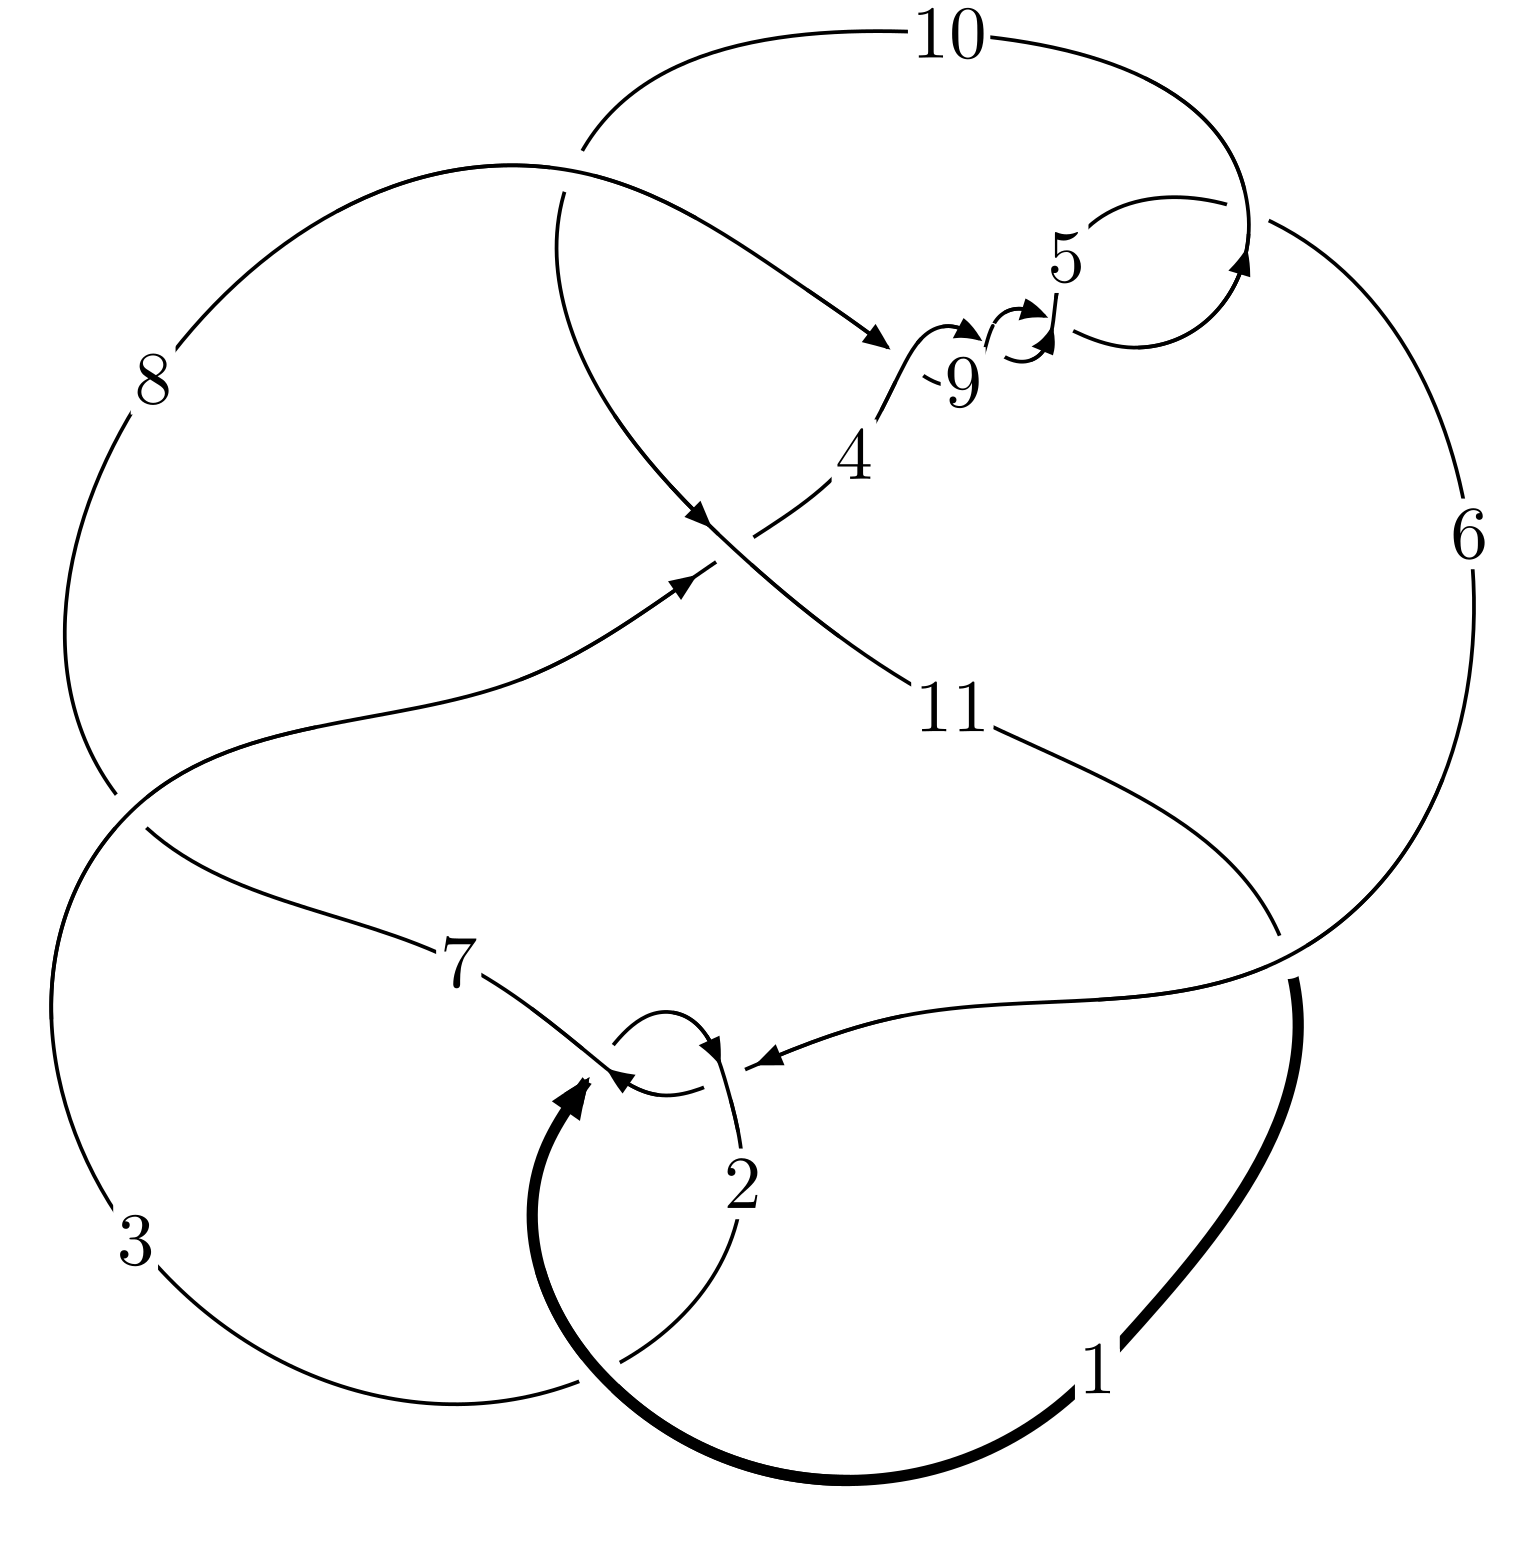
\includegraphics[width=112pt]{../../../GIT/diagram.site/Diagrams/png/433_11a_184.png}\\
\ \ \ A knot diagram\footnotemark}&
\allowdisplaybreaks
\textbf{Linearized knot diagam} \\
\cline{2-2}
 &
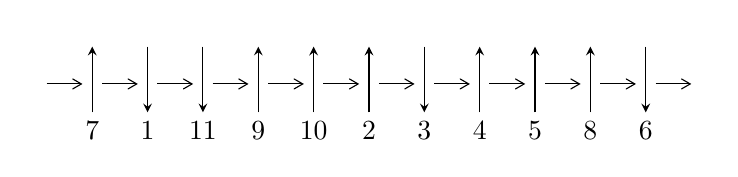
\begin{tikzpicture}[x=20pt, y=17pt]
	% nodes
	\node (C0) at (0, 0) {};
	\node (C1) at (1, 0) {};
	\node (C1U) at (1, +1) {};
	\node (C1D) at (1, -1) {7};

	\node (C2) at (2, 0) {};
	\node (C2U) at (2, +1) {};
	\node (C2D) at (2, -1) {1};

	\node (C3) at (3, 0) {};
	\node (C3U) at (3, +1) {};
	\node (C3D) at (3, -1) {11};

	\node (C4) at (4, 0) {};
	\node (C4U) at (4, +1) {};
	\node (C4D) at (4, -1) {9};

	\node (C5) at (5, 0) {};
	\node (C5U) at (5, +1) {};
	\node (C5D) at (5, -1) {10};

	\node (C6) at (6, 0) {};
	\node (C6U) at (6, +1) {};
	\node (C6D) at (6, -1) {2};

	\node (C7) at (7, 0) {};
	\node (C7U) at (7, +1) {};
	\node (C7D) at (7, -1) {3};

	\node (C8) at (8, 0) {};
	\node (C8U) at (8, +1) {};
	\node (C8D) at (8, -1) {4};

	\node (C9) at (9, 0) {};
	\node (C9U) at (9, +1) {};
	\node (C9D) at (9, -1) {5};

	\node (C10) at (10, 0) {};
	\node (C10U) at (10, +1) {};
	\node (C10D) at (10, -1) {8};

	\node (C11) at (11, 0) {};
	\node (C11U) at (11, +1) {};
	\node (C11D) at (11, -1) {6};
	\node (C12) at (12, 0) {};

	% arrows
	\draw[->,>={angle 60}]
	(C0) edge (C1) (C1) edge (C2) (C2) edge (C3) (C3) edge (C4) (C4) edge (C5) (C5) edge (C6) (C6) edge (C7) (C7) edge (C8) (C8) edge (C9) (C9) edge (C10) (C10) edge (C11) (C11) edge (C12) ;	\draw[->,>=stealth]
	(C1D) edge (C1U) (C2U) edge (C2D) (C3U) edge (C3D) (C4D) edge (C4U) (C5D) edge (C5U) (C6D) edge (C6U) (C7U) edge (C7D) (C8D) edge (C8U) (C9D) edge (C9U) (C10D) edge (C10U) (C11U) edge (C11D) ;
	\end{tikzpicture} \\
\hhline{~~} \\& 
\textbf{Solving Sequence} \\ \cline{2-2} 
 &
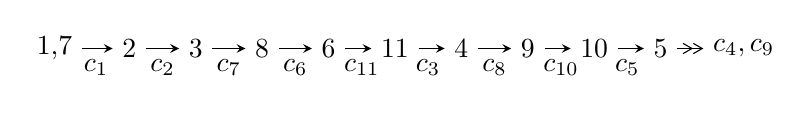
\begin{tikzpicture}[x=24pt, y=7pt]
	% node
	\node (A0) at (-1/8, 0) {1,7};
	\node (A1) at (1, 0) {2};
	\node (A2) at (2, 0) {3};
	\node (A3) at (3, 0) {8};
	\node (A4) at (4, 0) {6};
	\node (A5) at (5, 0) {11};
	\node (A6) at (6, 0) {4};
	\node (A7) at (7, 0) {9};
	\node (A8) at (8, 0) {10};
	\node (A9) at (9, 0) {5};
	\node (C1) at (1/2, -1) {$c_{1}$};
	\node (C2) at (3/2, -1) {$c_{2}$};
	\node (C3) at (5/2, -1) {$c_{7}$};
	\node (C4) at (7/2, -1) {$c_{6}$};
	\node (C5) at (9/2, -1) {$c_{11}$};
	\node (C6) at (11/2, -1) {$c_{3}$};
	\node (C7) at (13/2, -1) {$c_{8}$};
	\node (C8) at (15/2, -1) {$c_{10}$};
	\node (C9) at (17/2, -1) {$c_{5}$};
	\node (A10) at (41/4, 0) {$c_{4},c_{9}$};

	% edge
	\draw[->,>=stealth]	
	(A0) edge (A1) (A1) edge (A2) (A2) edge (A3) (A3) edge (A4) (A4) edge (A5) (A5) edge (A6) (A6) edge (A7) (A7) edge (A8) (A8) edge (A9) ;
	\draw[->>,>={angle 60}]	
	(A9) edge (A10);
\end{tikzpicture} \\ 

\end{tabular} \\

\footnotetext{
The image of knot diagram is generated by the software ``\textbf{Draw programme}" developed by Andrew Bartholomew(\url{http://www.layer8.co.uk/maths/draw/index.htm\#Running-draw}), where we modified some parts for our purpose(\url{https://github.com/CATsTAILs/LinksPainter}).
}\phantom \\ \newline 
\centering \textbf{Ideals for irreducible components\footnotemark of $X_{\text{par}}$} 
 
\begin{align*}
I^u_{1}&=\langle 
u^{43}- u^{42}+\cdots- u^2+1\rangle \\
\\
\end{align*}
\raggedright * 1 irreducible components of $\dim_{\mathbb{C}}=0$, with total 43 representations.\\
\footnotetext{All coefficients of polynomials are rational numbers. But the coefficients are sometimes approximated in decimal forms when there is not enough margin.}
\newpage
\renewcommand{\arraystretch}{1}
\centering \section*{I. $I^u_{1}= \langle u^{43}- u^{42}+\cdots- u^2+1 \rangle$}
\flushleft \textbf{(i) Arc colorings}\\
\begin{tabular}{m{7pt} m{180pt} m{7pt} m{180pt} }
\flushright $a_{1}=$&$\begin{pmatrix}1\\0\end{pmatrix}$ \\
\flushright $a_{7}=$&$\begin{pmatrix}0\\u\end{pmatrix}$ \\
\flushright $a_{2}=$&$\begin{pmatrix}1\\- u^2\end{pmatrix}$ \\
\flushright $a_{3}=$&$\begin{pmatrix}u^2+1\\- u^2\end{pmatrix}$ \\
\flushright $a_{8}=$&$\begin{pmatrix}- u^5-2 u^3- u\\u^5+u^3+u\end{pmatrix}$ \\
\flushright $a_{6}=$&$\begin{pmatrix}- u\\u^3+u\end{pmatrix}$ \\
\flushright $a_{11}=$&$\begin{pmatrix}u^4+u^2+1\\- u^6-2 u^4- u^2\end{pmatrix}$ \\
\flushright $a_{4}=$&$\begin{pmatrix}- u^{12}-3 u^{10}-5 u^8-4 u^6-2 u^4+u^2+1\\u^{14}+4 u^{12}+7 u^{10}+6 u^8+2 u^6- u^2\end{pmatrix}$ \\
\flushright $a_{9}=$&$\begin{pmatrix}- u^{31}-8 u^{29}+\cdots-12 u^7-4 u^5\\u^{33}+9 u^{31}+\cdots+4 u^7+u\end{pmatrix}$ \\
\flushright $a_{10}=$&$\begin{pmatrix}u^{16}+5 u^{14}+11 u^{12}+12 u^{10}+5 u^8-2 u^6-2 u^4+1\\- u^{16}-4 u^{14}-8 u^{12}-8 u^{10}-4 u^8\end{pmatrix}$ \\
\flushright $a_{5}=$&$\begin{pmatrix}- u^{35}-10 u^{33}+\cdots- u^3-2 u\\u^{35}+9 u^{33}+\cdots+u^3+u\end{pmatrix}$\\ \flushright $a_{5}=$&$\begin{pmatrix}- u^{35}-10 u^{33}+\cdots- u^3-2 u\\u^{35}+9 u^{33}+\cdots+u^3+u\end{pmatrix}$\\&\end{tabular}
\flushleft \textbf{(ii) Obstruction class $= -1$}\\~\\
\flushleft \textbf{(iii) Cusp Shapes $= -4 u^{41}+4 u^{40}-44 u^{39}+44 u^{38}-236 u^{37}+240 u^{36}-796 u^{35}+832 u^{34}-1848 u^{33}+2004 u^{32}-3040 u^{31}+3444 u^{30}-3480 u^{29}+4132 u^{28}-2468 u^{27}+3044 u^{26}-428 u^{25}+452 u^{24}+1264 u^{23}-1860 u^{22}+1600 u^{21}-2240 u^{20}+824 u^{19}-920 u^{18}-84 u^{17}+456 u^{16}-464 u^{15}+772 u^{14}-336 u^{13}+332 u^{12}-72 u^{11}-72 u^{10}+76 u^9-136 u^8+68 u^7-44 u^6+16 u^5+8 u^4-8 u^3+8 u^2-4 u+2$}\\~\\
\newpage\renewcommand{\arraystretch}{1}
\flushleft \textbf{(iv) u-Polynomials at the component}\newline \\
\begin{tabular}{m{50pt}|m{274pt}}
Crossings & \hspace{64pt}u-Polynomials at each crossing \\
\hline $$\begin{aligned}c_{1},c_{6}\end{aligned}$$&$\begin{aligned}
&u^{43}+u^{42}+\cdots+u^2-1
\end{aligned}$\\
\hline $$\begin{aligned}c_{2}\end{aligned}$$&$\begin{aligned}
&u^{43}+23 u^{42}+\cdots+2 u-1
\end{aligned}$\\
\hline $$\begin{aligned}c_{3}\end{aligned}$$&$\begin{aligned}
&u^{43}-5 u^{42}+\cdots-2 u+5
\end{aligned}$\\
\hline $$\begin{aligned}c_{4},c_{5},c_{8}\\c_{9}\end{aligned}$$&$\begin{aligned}
&u^{43}+u^{42}+\cdots+u^2-1
\end{aligned}$\\
\hline $$\begin{aligned}c_{7},c_{11}\end{aligned}$$&$\begin{aligned}
&u^{43}- u^{42}+\cdots-5 u-2
\end{aligned}$\\
\hline $$\begin{aligned}c_{10}\end{aligned}$$&$\begin{aligned}
&u^{43}+11 u^{42}+\cdots+12 u+1
\end{aligned}$\\
\hline
\end{tabular}\\~\\
\newpage\renewcommand{\arraystretch}{1}
\flushleft \textbf{(v) Riley Polynomials at the component}\newline \\
\begin{tabular}{m{50pt}|m{274pt}}
Crossings & \hspace{64pt}Riley Polynomials at each crossing \\
\hline $$\begin{aligned}c_{1},c_{6}\end{aligned}$$&$\begin{aligned}
&y^{43}+23 y^{42}+\cdots+2 y-1
\end{aligned}$\\
\hline $$\begin{aligned}c_{2}\end{aligned}$$&$\begin{aligned}
&y^{43}-5 y^{42}+\cdots+14 y-1
\end{aligned}$\\
\hline $$\begin{aligned}c_{3}\end{aligned}$$&$\begin{aligned}
&y^{43}+7 y^{42}+\cdots-926 y-25
\end{aligned}$\\
\hline $$\begin{aligned}c_{4},c_{5},c_{8}\\c_{9}\end{aligned}$$&$\begin{aligned}
&y^{43}-49 y^{42}+\cdots+2 y-1
\end{aligned}$\\
\hline $$\begin{aligned}c_{7},c_{11}\end{aligned}$$&$\begin{aligned}
&y^{43}-33 y^{42}+\cdots+125 y-4
\end{aligned}$\\
\hline $$\begin{aligned}c_{10}\end{aligned}$$&$\begin{aligned}
&y^{43}- y^{42}+\cdots-18 y-1
\end{aligned}$\\
\hline
\end{tabular}\\~\\
\newpage\flushleft \textbf{(vi) Complex Volumes and Cusp Shapes}
$$\begin{array}{c|c|c}  
\text{Solutions to }I^u_{1}& \I (\text{vol} + \sqrt{-1}CS) & \text{Cusp shape}\\
 \hline 
\begin{aligned}
u &= \phantom{-}0.521315 + 0.837611 I\end{aligned}
 & \phantom{-}1.91297 + 4.88049 I & \phantom{-}7.17506 - 8.80545 I \\ \hline\begin{aligned}
u &= \phantom{-}0.521315 - 0.837611 I\end{aligned}
 & \phantom{-}1.91297 - 4.88049 I & \phantom{-}7.17506 + 8.80545 I \\ \hline\begin{aligned}
u &= -0.564675 + 0.846085 I\end{aligned}
 & \phantom{-}9.73939 - 6.81501 I & \phantom{-}9.15243 + 6.58080 I \\ \hline\begin{aligned}
u &= -0.564675 - 0.846085 I\end{aligned}
 & \phantom{-}9.73939 + 6.81501 I & \phantom{-}9.15243 - 6.58080 I \\ \hline\begin{aligned}
u &= -0.070971 + 0.949282 I\end{aligned}
 & -1.88710 - 1.49301 I & -2.49179 + 5.12316 I \\ \hline\begin{aligned}
u &= -0.070971 - 0.949282 I\end{aligned}
 & -1.88710 + 1.49301 I & -2.49179 - 5.12316 I \\ \hline\begin{aligned}
u &= \phantom{-}0.157033 + 1.039100 I\end{aligned}
 & \phantom{-}4.88985 + 3.07247 I & \phantom{-}2.04876 - 3.22790 I \\ \hline\begin{aligned}
u &= \phantom{-}0.157033 - 1.039100 I\end{aligned}
 & \phantom{-}4.88985 - 3.07247 I & \phantom{-}2.04876 + 3.22790 I \\ \hline\begin{aligned}
u &= -0.443218 + 0.795583 I\end{aligned}
 & \phantom{-}0.18390 - 1.87415 I & \phantom{-}2.36398 + 3.86442 I \\ \hline\begin{aligned}
u &= -0.443218 - 0.795583 I\end{aligned}
 & \phantom{-}0.18390 + 1.87415 I & \phantom{-}2.36398 - 3.86442 I \\ \hline\begin{aligned}
u &= -0.578652 + 0.674431 I\end{aligned}
 & \phantom{-}10.22700 + 2.27386 I & \phantom{-}10.59990 + 0.05953 I \\ \hline\begin{aligned}
u &= -0.578652 - 0.674431 I\end{aligned}
 & \phantom{-}10.22700 - 2.27386 I & \phantom{-}10.59990 - 0.05953 I \\ \hline\begin{aligned}
u &= \phantom{-}0.509969 + 0.679497 I\end{aligned}
 & \phantom{-}2.36364 - 0.64965 I & \phantom{-}9.29098 + 1.48220 I \\ \hline\begin{aligned}
u &= \phantom{-}0.509969 - 0.679497 I\end{aligned}
 & \phantom{-}2.36364 + 0.64965 I & \phantom{-}9.29098 - 1.48220 I \\ \hline\begin{aligned}
u &= \phantom{-}0.802703 + 0.162351 I\end{aligned}
 & \phantom{-}6.46390 - 7.57490 I & \phantom{-}7.29481 + 4.51486 I \\ \hline\begin{aligned}
u &= \phantom{-}0.802703 - 0.162351 I\end{aligned}
 & \phantom{-}6.46390 + 7.57490 I & \phantom{-}7.29481 - 4.51486 I \\ \hline\begin{aligned}
u &= -0.783539 + 0.138077 I\end{aligned}
 & -1.13687 + 5.20298 I & \phantom{-}4.40416 - 6.22689 I \\ \hline\begin{aligned}
u &= -0.783539 - 0.138077 I\end{aligned}
 & -1.13687 - 5.20298 I & \phantom{-}4.40416 + 6.22689 I \\ \hline\begin{aligned}
u &= \phantom{-}0.495820 + 1.104130 I\end{aligned}
 & \phantom{-}6.52652 + 3.46599 I & \phantom{-}6.43711 - 3.77434 I \\ \hline\begin{aligned}
u &= \phantom{-}0.495820 - 1.104130 I\end{aligned}
 & \phantom{-}6.52652 - 3.46599 I & \phantom{-}6.43711 + 3.77434 I \\ \hline\begin{aligned}
u &= -0.781151\phantom{ +0.000000I}\end{aligned}
 & \phantom{-}2.55363\phantom{ +0.000000I} & \phantom{-}4.52390\phantom{ +0.000000I} \\ \hline\begin{aligned}
u &= \phantom{-}0.758021 + 0.099035 I\end{aligned}
 & -2.34232 - 1.57976 I & \phantom{-}0.847135 + 0.282398 I \\ \hline\begin{aligned}
u &= \phantom{-}0.758021 - 0.099035 I\end{aligned}
 & -2.34232 + 1.57976 I & \phantom{-}0.847135 - 0.282398 I \\ \hline\begin{aligned}
u &= -0.463782 + 1.145440 I\end{aligned}
 & -1.69075 - 3.98657 I & \phantom{-}4.72929 + 3.11894 I \\ \hline\begin{aligned}
u &= -0.463782 - 1.145440 I\end{aligned}
 & -1.69075 + 3.98657 I & \phantom{-}4.72929 - 3.11894 I \\ \hline\begin{aligned}
u &= -0.382526 + 1.197980 I\end{aligned}
 & -5.08887 + 1.28085 I & \phantom{-0.000000 } 0. - 2.90376 I \\ \hline\begin{aligned}
u &= -0.382526 - 1.197980 I\end{aligned}
 & -5.08887 - 1.28085 I & \phantom{-0.000000 -}0. + 2.90376 I \\ \hline\begin{aligned}
u &= \phantom{-}0.362492 + 1.206110 I\end{aligned}
 & \phantom{-}2.33692 - 3.70518 I & \phantom{-}2.48681 + 1.54084 I \\ \hline\begin{aligned}
u &= \phantom{-}0.362492 - 1.206110 I\end{aligned}
 & \phantom{-}2.33692 + 3.70518 I & \phantom{-}2.48681 - 1.54084 I \\ \hline\begin{aligned}
u &= \phantom{-}0.407336 + 1.191840 I\end{aligned}
 & -6.07657 + 2.44102 I & -3.16979 - 3.57779 I\\
 \hline 
 \end{array}$$\newpage$$\begin{array}{c|c|c}  
\text{Solutions to }I^u_{1}& \I (\text{vol} + \sqrt{-1}CS) & \text{Cusp shape}\\
 \hline 
\begin{aligned}
u &= \phantom{-}0.407336 - 1.191840 I\end{aligned}
 & -6.07657 - 2.44102 I & -3.16979 + 3.57779 I \\ \hline\begin{aligned}
u &= -0.448865 + 1.200600 I\end{aligned}
 & -0.96199 - 4.39851 I & \phantom{-0.000000 -}0. + 3.54146 I \\ \hline\begin{aligned}
u &= -0.448865 - 1.200600 I\end{aligned}
 & -0.96199 + 4.39851 I & \phantom{-0.000000 } 0. - 3.54146 I \\ \hline\begin{aligned}
u &= \phantom{-}0.490454 + 1.184460 I\end{aligned}
 & -5.48574 + 6.18515 I & -2.04828 - 3.59368 I \\ \hline\begin{aligned}
u &= \phantom{-}0.490454 - 1.184460 I\end{aligned}
 & -5.48574 - 6.18515 I & -2.04828 + 3.59368 I \\ \hline\begin{aligned}
u &= \phantom{-}0.645564 + 0.300310 I\end{aligned}
 & \phantom{-}8.84662 + 0.96374 I & \phantom{-}10.02944 - 0.37589 I \\ \hline\begin{aligned}
u &= \phantom{-}0.645564 - 0.300310 I\end{aligned}
 & \phantom{-}8.84662 - 0.96374 I & \phantom{-}10.02944 + 0.37589 I \\ \hline\begin{aligned}
u &= -0.507296 + 1.186730 I\end{aligned}
 & -4.20932 - 9.96665 I & \phantom{-0.000000 -}0. + 9.16746 I \\ \hline\begin{aligned}
u &= -0.507296 - 1.186730 I\end{aligned}
 & -4.20932 + 9.96665 I & \phantom{-0.000000 } 0. - 9.16746 I \\ \hline\begin{aligned}
u &= \phantom{-}0.519799 + 1.187960 I\end{aligned}
 & \phantom{-}3.43954 + 12.44990 I & \phantom{-}4.17518 - 7.63100 I \\ \hline\begin{aligned}
u &= \phantom{-}0.519799 - 1.187960 I\end{aligned}
 & \phantom{-}3.43954 - 12.44990 I & \phantom{-}4.17518 + 7.63100 I \\ \hline\begin{aligned}
u &= -0.536405 + 0.171930 I\end{aligned}
 & \phantom{-}1.103730 - 0.098765 I & \phantom{-}9.44099 + 0.91027 I \\ \hline\begin{aligned}
u &= -0.536405 - 0.171930 I\end{aligned}
 & \phantom{-}1.103730 + 0.098765 I & \phantom{-}9.44099 - 0.91027 I\\
 \hline 
 \end{array}$$\newpage
\newpage\renewcommand{\arraystretch}{1}
\centering \section*{ II. u-Polynomials}
\begin{tabular}{m{50pt}|m{274pt}}
Crossings & \hspace{64pt}u-Polynomials at each crossing \\
\hline $$\begin{aligned}c_{1},c_{6}\end{aligned}$$&$\begin{aligned}
&u^{43}+u^{42}+\cdots+u^2-1
\end{aligned}$\\
\hline $$\begin{aligned}c_{2}\end{aligned}$$&$\begin{aligned}
&u^{43}+23 u^{42}+\cdots+2 u-1
\end{aligned}$\\
\hline $$\begin{aligned}c_{3}\end{aligned}$$&$\begin{aligned}
&u^{43}-5 u^{42}+\cdots-2 u+5
\end{aligned}$\\
\hline $$\begin{aligned}c_{4},c_{5},c_{8}\\c_{9}\end{aligned}$$&$\begin{aligned}
&u^{43}+u^{42}+\cdots+u^2-1
\end{aligned}$\\
\hline $$\begin{aligned}c_{7},c_{11}\end{aligned}$$&$\begin{aligned}
&u^{43}- u^{42}+\cdots-5 u-2
\end{aligned}$\\
\hline $$\begin{aligned}c_{10}\end{aligned}$$&$\begin{aligned}
&u^{43}+11 u^{42}+\cdots+12 u+1
\end{aligned}$\\
\hline
\end{tabular}\newpage\renewcommand{\arraystretch}{1}
\centering \section*{ III. Riley Polynomials}
\begin{tabular}{m{50pt}|m{274pt}}
Crossings & \hspace{64pt}Riley Polynomials at each crossing \\
\hline $$\begin{aligned}c_{1},c_{6}\end{aligned}$$&$\begin{aligned}
&y^{43}+23 y^{42}+\cdots+2 y-1
\end{aligned}$\\
\hline $$\begin{aligned}c_{2}\end{aligned}$$&$\begin{aligned}
&y^{43}-5 y^{42}+\cdots+14 y-1
\end{aligned}$\\
\hline $$\begin{aligned}c_{3}\end{aligned}$$&$\begin{aligned}
&y^{43}+7 y^{42}+\cdots-926 y-25
\end{aligned}$\\
\hline $$\begin{aligned}c_{4},c_{5},c_{8}\\c_{9}\end{aligned}$$&$\begin{aligned}
&y^{43}-49 y^{42}+\cdots+2 y-1
\end{aligned}$\\
\hline $$\begin{aligned}c_{7},c_{11}\end{aligned}$$&$\begin{aligned}
&y^{43}-33 y^{42}+\cdots+125 y-4
\end{aligned}$\\
\hline $$\begin{aligned}c_{10}\end{aligned}$$&$\begin{aligned}
&y^{43}- y^{42}+\cdots-18 y-1
\end{aligned}$\\
\hline
\end{tabular}
\vskip 2pc
\end{document}